\documentclass[11pt, a4paper, oneside]{book}
\usepackage[utf8]{inputenc}
\usepackage[backend=bibtex, style=ieee]{biblatex}
\bibliography{references} %Imports bibliography file
% Packages validated to be needed
\usepackage{graphicx}       % for minipage
\usepackage{amsmath}        % for align*
\usepackage{indentfirst}    % for indenting paragraphs after titles
\usepackage{fancyhdr}       % For modifying header style and or size
\usepackage{titlesec}       % For removing 'chapter N' from section titles
\usepackage{setspace}       % Used for double spacing
\usepackage{subfigure}      % For figure placement
\usepackage{wrapfig}        % For wrapping figures
\usepackage{textcomp}       % For copyright symbol
\usepackage{tabularx}       % For controlling width of the table
\usepackage{hhline}         % For the double lines in the table
% \usepackage[mark=***]{sectionbreak} % For a section break
% \usepackage[left=35mm, right=35mm, top=35, bottom=35]{geometry} % For setting margin width
%
\titleformat{\chapter}[display]{\normalfont\huge\bfseries}{}{0pt}{\Huge}        % For removing 'chapter N' from titlesec
\titlespacing*{\chapter} {0pt}{0pt}{40pt}      % For removing 'chapter N' from titlesec
\doublespacing          % double spacing from setspace

\usepackage{microtype}

\usepackage[english]{babel}
%Includes "References" in the table of contents
\usepackage[nottoc]{tocbibind}
%\usepackage[ngerman]{babel}
\usepackage{csquotes}
\usepackage{subcaption}
\usepackage[hidelinks]{hyperref}

\usepackage{acronym}
\usepackage{graphicx}
\graphicspath{ {./images/} }



\usepackage{xspace}
\usepackage{mdframed}
\usepackage{color, colortbl}
\usepackage{array}
\newcolumntype{L}[1]{>{\RaggedRight\hsize=#1\hsize\linewidth=\hsize}X}
\usepackage{booktabs}


%\linespread{0.4}

\def\paperType{Honors Thesis}
\def\title{Modeling Sea Ice Thickness using Machine Learning and Remote Sensing Modalities}
\def\honorsCollege{Barrett, The Honors College}
\def\collegeOfMajor{Ira A. Fulton Schools of Engineering}
\def\schoolOfMajor{School of Computing and Augmented Intelligence}
\def\author{John Baker}
\def\director{Dr.~Douglas Cochran}
\def\secondReader{Dr.~Hua Wei}
%\def\addrLineEins{Thesis Time Period}
\def\majorOfStudy{Study Program}
\def\studentId{1234567890}
%\def\semester{Insert Semester and Academic Year}

\def\location{Duisburg}
\def\date{Month, Year}
\setlength\parindent{24pt}


\begin{document}
    % !TeX root = main.tex

\begin{titlepage}
	\vspace*{-6em}
	\hspace{-3.5em}
	\vspace*{\fill}
			
	\begin{center}
		\vspace*{\fill}
		%Thesis Title\\
		%\vspace*{\fill}
		{\huge\bfseries \title} \\
    \vspace{1cm}
	 	\author	\\
   	\collegeOfMajor \\
   	\schoolOfMajor
		\vspace*{\fill}
		%\vspace*{\fill}
		%\\
		\vspace*{\fill}
		%\addrLineEins\\

	\end{center}
	\vspace*{\fill}

\begin{minipage}[][5cm][b]{\textwidth}
\begin{align*}
&\textsc{Approved:}\\[.5cm]
&\quad\textrm{\director} &\underline{\hspace{6cm}},\qquad &\textrm{Director}\\[.5cm]
&\quad\textrm{\secondReader} &\underline{\hspace{6cm}}, \qquad &\textrm{Second Reader}\\[.5cm]
\end{align*}
\begin{flushright}
\textsc{Accepted:} \\[1.0cm]
\underline{\hspace{6.0cm}}\\
Dean, Barrett, the Honors College\\
\end{flushright}
\end{minipage}\\
~

\end{titlepage}
    % This is an example of the thesis outline. Please adapt this template to fit your needs.
	% !TeX root = main.tex

\begin{titlepage}
	\center
	\begin{singlespace}
	
	\textsc{\huge Arizona State University} \\[1.5cm]
	
	\rule{\textwidth}{1.6pt}\vspace*{-\baselineskip}\vspace*{2pt}
	\rule{\textwidth}{0.4pt}\\[\baselineskip] % thin horizontal line
	\vspace{-.5cm}{\Huge \title\\[0.3cm] }% Title
	
	\rule{\textwidth}{0.4pt}\vspace*{-\baselineskip}\vspace{3.2pt} % Thin horizontal line
	\rule{\textwidth}{1.6pt}\\[1.5cm] % Thick horizontal line
	
	
	\textsc{\Large \paperType} \\[0.2cm]
	\textsc{\normalsize \honorsCollege} \\[2.5cm]
	\vspace{.5cm}
	
	
	\emph{\Large Author:}\\[0.25cm]
	{\Large \author} \\[2cm] 
	\emph{\Large Committee:}\\[0.25cm]
	{\Large \director \\[0.2cm] \secondReader} \\[2.5cm]
	
	{\Large April 2024}
	\end{singlespace}
	
	\end{titlepage}

    % !TeX root = main.tex

\chapter*{Acknowledgement}
I hereby declare that I can carry out the present work independently without outside help.
and used only the sources and aids indicated. I assure
Furthermore, that I have not yet submitted this thesis to any other examination board.



\vspace{5em}

    % !TeX root = main.tex

\thispagestyle{empty}

\chapter*{Abstract}
English Abstract here. The abstract should provide a complete but concise description of your work. In brief, you should address the following: motivation, problem statement, approach, results, and conclusions. 


% {\let\clearpage\relax \chapter*{Zusammenfassung}}
% Deutsche Zusammenfassung hier. 



    \begin{onehalfspace}
    \tableofcontents
	\end{onehalfspace}

    \clearpage
    
    \chapter{Introduction}
\label{sec:Introduction}

\paragraph{}
A distinct problem arising from attempting to study the exact state of sea ice is that there is limited data available. Data pertaining to sea ice is widely distributed, not correlated, or limited in scope such that it's difficult to draw inferences from. Naturally, the immediate approach to this thesis will first require research into available data sources before conducting any exploration. This exploration will reveal which sources should be targeted for the remainder of the thesis.

\indent After reviewing the preliminary research, this paper will move forward to a more targeted effort in obtaining and analyzing data to develop a machine learning model that can be used to predict ice thickness from said remote sensing methods. Chapter 2 will describe the process of obtaining the selected data, and Chapter 3 will discuss the methodology of developing the model.
\par

\section{Preliminary Research}
Preliminary research into the availability of ice thickness data yields three notable organizations which may act as sources of data. These three organizations are the National Snow and Ice Data Center (NSIDC), the National Aeronautics and Space Administration (NASA), and the European Space Agency (ESA). Although all organizations offer large amounts of data, they differ in approach. The NSIDC acts as a historic repository, accumulating previous studies into a single location for easy access. NASA offers a similar service, but additionally allows researchers the opportunity to query information from any of their active orbiting satellites. The ESA, like NASA, offers near real-time satellite data but also offers to sponsor data from external companies with the completion of a project proposal.

\subsection*{NSIDC}
Here is where the NSIDC links and data retrieval should be discussed. Limitations of the data or other notes about it's composition should be included according to the details in the abstract saved on file. Preliminary exploration will be where the figures will be uploaded (Or maybe we show one figure showing all of the points, and the exploration will be for the single instance?)

\subsection*{ESA}
Here is where you discuss the ESA's copernicus portal, finding the ICEYE company, looking through the proposal process, seeing superior SAR resolution from this private company than NASA's sentinel-2

\subsection*{NASA}
Here is where you should include sources to the ATL10 Data Specification pdf, and the associated CryoSat data specs. It should also be included where these links came from. It also should be included where, if applicable, specific data downloads were from. It should include the process of querying for data, which portals are made accessible, and how flexible they are. Do not forget to mention that they made an IceSat-2 mobile application for iOS. \cite{ICESat-2-ATL10-Product}

Include how NASA's Sentinel-2 delivers SAR imaging, but at 50m resolution. This is a modality that can be used for a CNN but the resolution is not meaningfully compatible with any source of ground truth we have. Thus, searching for alternatives led to the European Space Agency and its sponsorship for ICEYE's 1m resolution imaging.

Somewhere you should discuss IceSat-2 and its laser altimetry. ESPECIALLY that it's 17m footprint offers precision at a given location, 

\section {Preliminary Exploration}
After researching the available data sources across these 3 agencies, the NSIDC's In-Situ dataset offered the greatest possibility of learning direct trends of sea ice. However, NASA's IceSat-2's predictable orbit combined with the possibility of obtaining ICEYE's high resolution SAR imaging, suggested that a temporally and spatially coincident dataset could be obtained. This intersection of remote sensed imagery with precise remotely sensed freeboard measurements, is conducive for a convolutional neural network applying IceSat-2's accuracy onto the expansiveness of SAR imaging. This model would be more dynamic in nature than the static accumulation of In-situ data, and would give more insight into the changing state of sea-ice. \cite{In-Situ-Dataset}

Importantly, it's important to recognize that laser altimetry is purely restricted to measuring Earth's surface - meaning the returned measurements are innately incapable of measuring sea-ice thickness, especially in the presence of snow on the surface. (Add source and put it in bibliography)
\begin{figure}[htb]
	\centering
	\subfigure{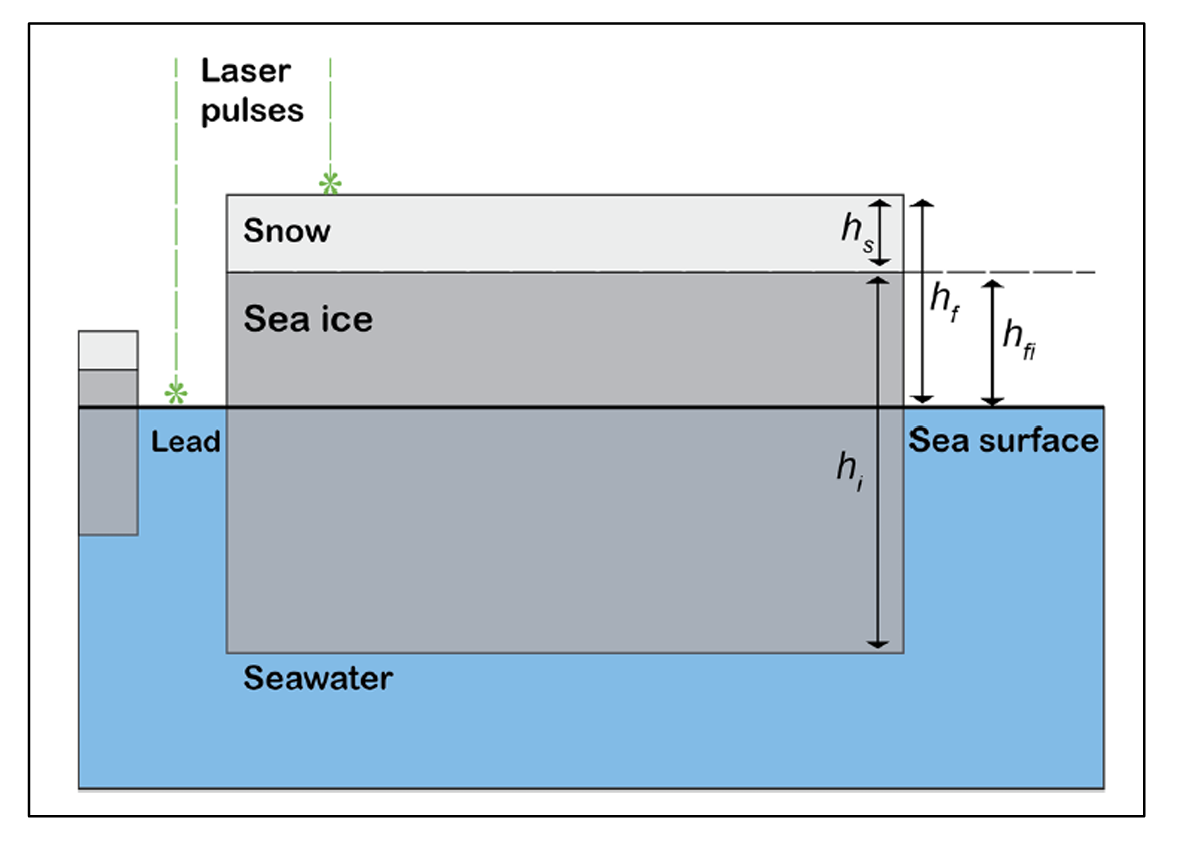
\includegraphics[width=.8\textwidth]{../research-resources/ice-sat-2/hydro-static-equillibrium.png}} 
	\caption{Laser Altimetry on a buoyant surface} \cite{ICESat-2-L4-Product}
	\label{fig:hydro-static-diagram}
\end{figure}

NASA's ICESat-2 L4 Along-Track Sea Ice Thickness highlights this problem, and addresses it using the assumption of hydro-static equilibrium. This equation, expressed as follows, uses the densities of water, sea-ice and snow, alongside the height of the snow to calculate the correlated thickness of the sea ice.

\begin{equation*}
	\rho_i
	\rho_w
	\rho_s
\end{equation*}

% Data of interest were the IceSat-2 ATL10 product and the NSIDC In-situ Dataset, selected for their combination of breadth and accuracy. Furthermore, the European Space Agency's requirements for sponsored data need to be explored to pursue the higher resolution SAR imagery hoped for. The in-situ measurements will provide an invaluable source of ground truth while the ATL10 product will drastically expand the flexibility and accessibility of sea ice freeboard data moving forward.

\subsection*{NSIDC}
\paragraph*{}
The "On-Ice Arctic Sea Ice Thickness Measurements by Auger, Core, and Electromagnetic Induction, from the Late 1800s Onward, Version 2" contains 69,750 rows of data, spanning 5 categorized regions; the Arctic Ocean, the Beaufort Sea, Greenland Coast, Prudhoe Bay, and Russian Coast. Filtering down to the Beaufort Sea region, a region of interest, yields 23 separate studies ranging between 1958 and 2016.
\par
%%% Modify which figures you're showing and in what order. It's not apparent what direction you're trying to go from here if you leave all 3 together like this.
\begin{figure}[htb]
	\centering
	\subfigure{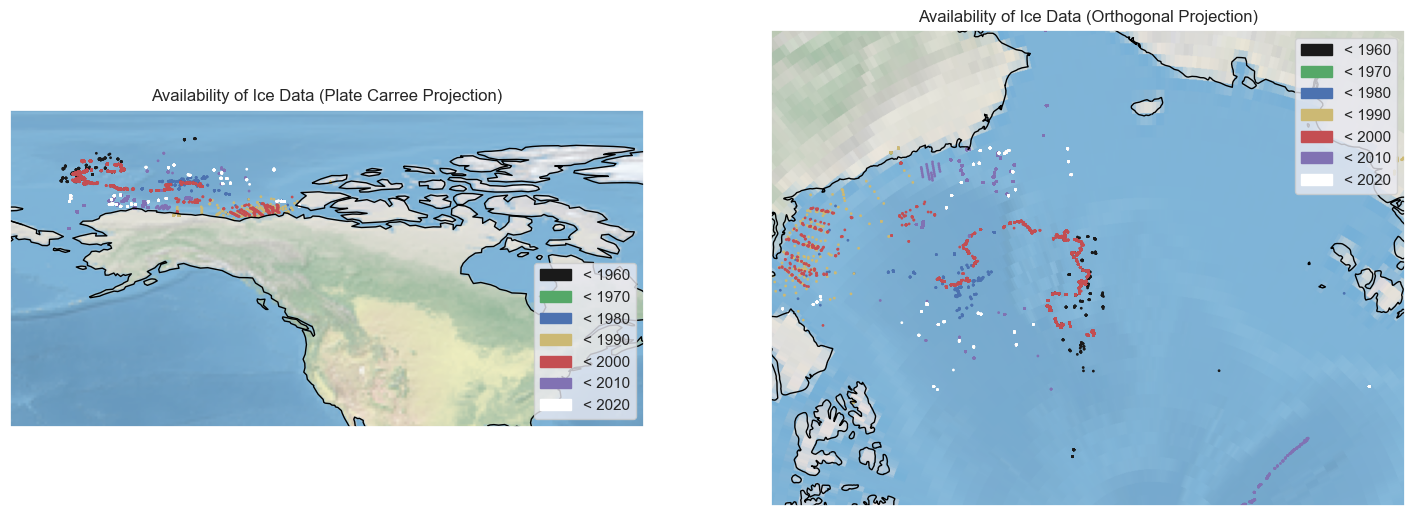
\includegraphics[width=0.8\textwidth]{../research-resources/in-situ/Plotted-Tracks.png}} 
	\subfigure{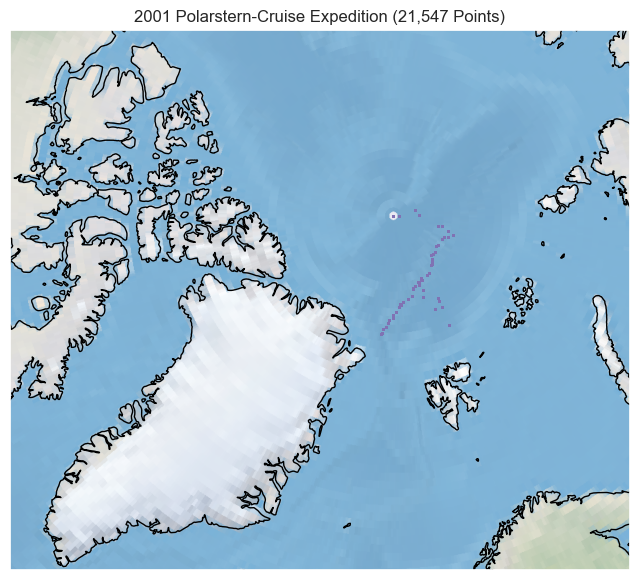
\includegraphics[width=0.5\textwidth]{../research-resources/in-situ/region-of-interest.png}} 
	\caption{In-Situ Data Availability}
	\label{fig:foobar}
\end{figure}


\paragraph*{}
For a simple analysis, the largest single dataset was chosen to conduct a simple test on the distribution of sea ice thickness. This distribution if normal will reasonably allow for future conducting of statistical tests, and if not normal will give insight as to what a reasonable assumption of ice thickness distribution should be. The largest dataset consists of 21,547 distinct points sourced from direct auger measurements and indirect electromagnetically sensed methods. Given that the majority of the data comes from the remote sensed method, it was validated by plotting the sensed values against the auger values where applicable and seeing how correlated they were. The results of a linear regression test yielded a relationship of 0.92x + 0.18, with an adjusted R\^2 value of 0.866 and a P Value of 2.31 * 10\^-202. The adjusted R\^2 value and low P value demonstrate there is a high correlation between these variables, and our model captures a significant portion of the variance. The 0 line is plotted as a way to visualize how the residuals are symmetrically clustered around 0.
\par

\begin{figure}[htb]
	\centering
	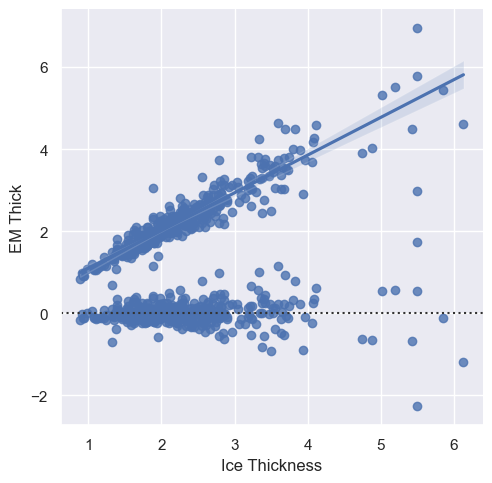
\includegraphics[width=.6\linewidth]{../research-resources/in-situ/auger-vs-em-thickness.png}
	\caption{Electromagnetic vs Auger Sourced Relationship}
	\label{fig:aug-vs-em}
\end{figure}

\paragraph*{}
After accepting the validity of the electromagnetically sensed data, the points were plotted to visualize the strip of ice that was measured. Given that these data points were taken in a single linear track, the line graph shows a cross-sectional profile of ice in that axis. The distribution reveals a slight tail on the left side of the curve, and a hypothesis test confirms that the distribution is not normal. Moving forward, it is reasonable to believe that ice distribution is not normal, and over a large enough sample there is expected to be a slight tail on either end.
\par
\begin{figure}[htb]
	\centering
	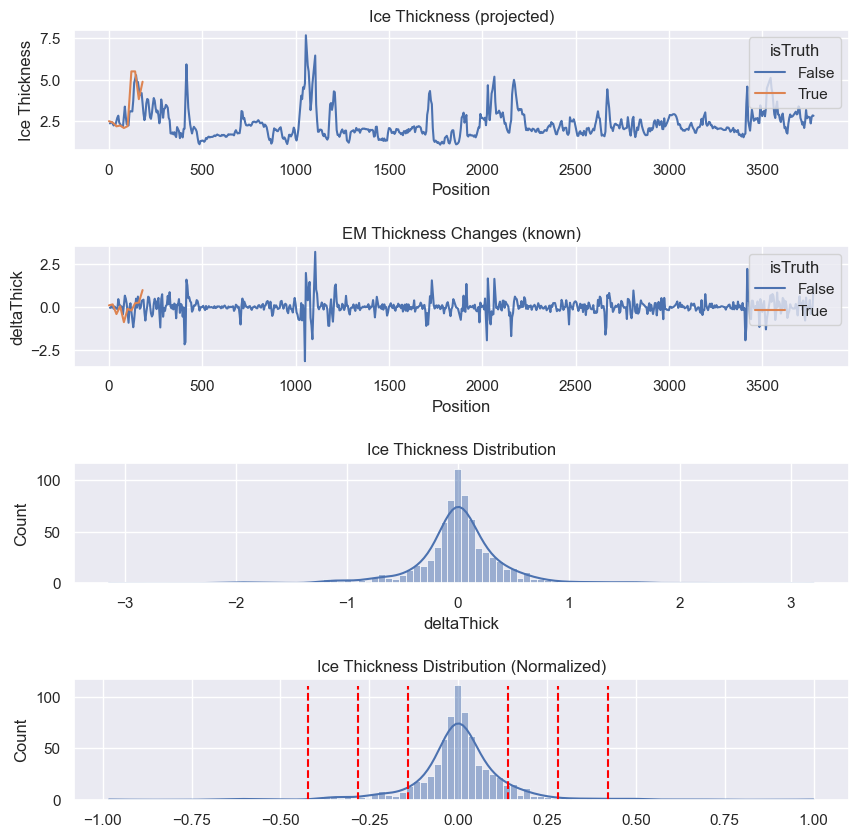
\includegraphics[width=\linewidth]{../research-resources/in-situ/track-graphs-p-test.png}
	\caption{In-Situ Ice Thickness Distribution}
	\label{fig:p-test-aug}
\end{figure}

\subsection*{NASA}
A single delivery of IceSat-2's ATL10 data product yields a '.h5' file, incompatible with traditional spreadsheets. To access IceSat-2 data in a meaningful way involved developing a script to extract relevant information according to the types enumerated in the data product specification. Columns of interest include the latitude, longitude, time, and calculated freeboard height for each of the three beam pairs.
// Consider adding perl and dynamically adding sample rows from the extracted .h5 file. This will give the reader context as to what's being gathered /


\subsection*{ESA}
Filling out the proposal for ICEYE sponsored data. (eg: See Appendix A or something)
    \chapter{Data Collection}
\label{sec:Data_Collection}

  
In this section, include research relevant to the gathering of data. Include the different metrics that may be captured and the different options presented from different avenues. Much research was done earlier based on the opportunities and limitations of NASA satellites. Include documentation you captured about CryoSat if pertinent to this section.

It may be necessary to include information on SAR imaging in the introduction, so even the non-expert reader can get a functional understanding of the topic.

It may be possible to include figures and other data from the NSIDC In-Situ data repository and discuss the viability of that data as a 'ground-truth' and demonstrate that according to those studies, sea ice was non-normal in distribution. Acknowledge that the data from those studies spanned many miles, and the distribution may sheerly be by variance of ice thickness across the collection area.

Here is where we'll discuss the selection of ICEYE's Data for it's high resolution imaging, and IceSat-2 for it's high-accuracy laser altimetry. It may be possible to include figures to demonstrate how these satellites work, but it may not be pertinent to the thesis (although it would help with understanding).

\section {Laser Altimetry (IceSat-2)}

\section {SAR Imaging (ICEYE)}

------Default Text ----------

Provide in brief the background information for your work/field keeping in mind that maybe your readers do not have experience with topics your reference or address in your thesis. 

In the second part, provide a review of the state of the art relevant to your thesis. Here you present relevant research that relates to your work. 

    \chapter{Experimentation}
\label{sec:Experimentation}

The intuition behind developing a CNN on this dataset is novel. Many related works demonstrate the feasibility of using CNN models to classify or segment SAR imaging \cite{SAR-U-Net}, but tend not to explore regression tasks. This could be a result of minimal data like the set derived for this study being accessible to the public. Furthermore, attempting to relate IS-2 footprints to high resolution SAR imaging involves deriving information from single-channel imagery of low pixel dimension. Compounded with the 33$\%$ yield of anticipated data from the ICEYE image, the limited data problem is exacerbated. 

\section{Setup}
The coincident data is first extracted from the ICEYE imagery, yielding 4,683 17x17 tiles with associated LiDAR measurements. The selected densities used for interpolation are as follows, where the snow density is drawn from historical measurements during the month of January \cite{warren1999snow}.

\begin{figure}[h]
  \[
  \begin{aligned}[t]
    \rho_i &=  \text{Density of sea ice }(916 \frac{kg}{m^3}) \\   %	It'd be perfect to place the diagram of the sheet in the white space generated here in latex
    \rho_s &=  \text{Density of snow }(300 \frac{kg}{m^3}) \\   %	It'd be perfect to place the diagram of the sheet in the white space generated here in latex
    \rho_w &=  \text{Density of water }(1024 \frac{kg}{m^3}) \\   %	It'd be perfect to place the diagram of the sheet in the white space generated here in latex
  \end{aligned}
\]
\end{figure}
  
Using Equation 1.1, each tile's elevation readings are converted to their associated thickness. Some values of freeboard are negative, so they are interpreted to represent the absence of snow and an overestimate of sea ice surface elevation. The negative freeboard values are then added to the sea ice surface elevation to compensate. Each tile's interpolated ice thickness can be visualized in Figure 3.1.

\begin{figure}[h!]
	\centering
	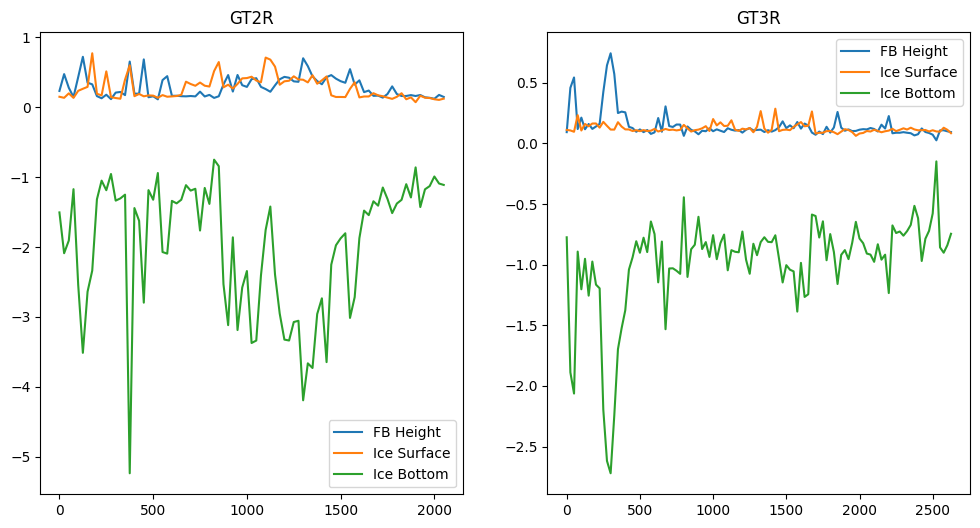
\includegraphics[width=\textwidth]{../research-resources/ice-sat-2/coincident-ice-profile.png}
	\caption{Interpolated Ice Thickness}
	\label{fig:ice-thickness-interpolation}
\end{figure}

The experimental model for the data is a feed forward neural network, consisting of 3 convolutional layers and 3 fully connected layers. Each convolutional layer is followed by the ReLU activation function, and the model uses the ADAM optimizer at a $10^{-5}$ learning rate based upon the L1 loss function. Given the already minimal pixel-space dimension, pooling and filter dilation are avoided to better preserve information across layers of the network.

The intuition behind experimenting with a simple model is rooted largely from the sparseness of existing studies attempting regression on low-resolution single channel images. Studies on classification, however, find that wider datasets (data that spans more classes) benefit from a larger amount of neurons in fully connected layers \cite{BASHA2020112}. Regression tasks for continuous numbers can be thought of as infinite classification, thus supporting the decision to implement multiple fully connected layers of large dimension. Some classification studies find value in decreasing filter sizes with model depth \cite{ganj2023lrnet}, but for this model, kernel size is decreased from 5 to 3 only between the first and second convolution layer.

\begin{figure}
  \centering
  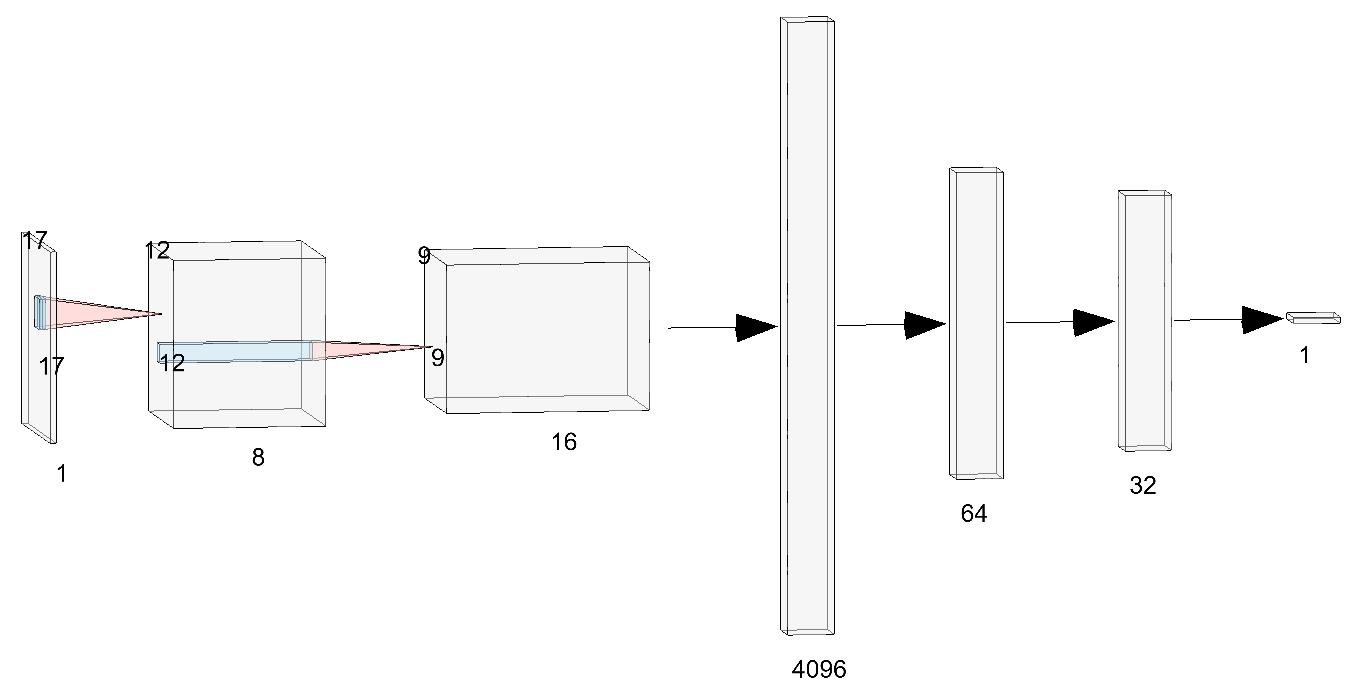
\includegraphics[width=0.8\textwidth]{../research-resources/CNN/model-architecture.png}
	\caption{CNN Architecture}
	\label{fig:cnn-model}
\end{figure}

The training process for the model uses 80\% of the data to train and 20\% to test, a batch size of 32 to promote faster convergence, random flipping and rotation to prevent over-fitting, and scaling of each pixel to the [0,255] color range. The model is trained over 100 epochs.


\section{Model Results}

\begin{figure}[hbt!]
	\centering
  \subfigure[]{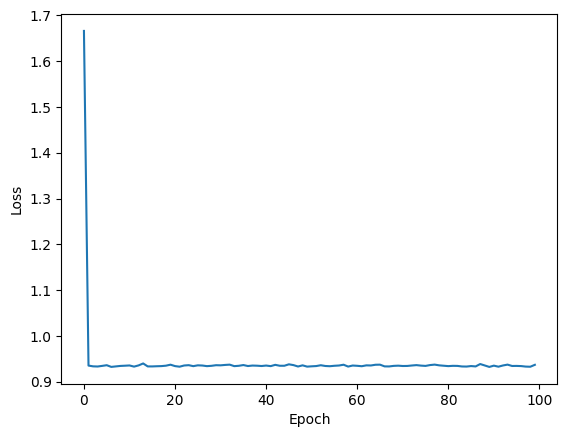
\includegraphics[width=.48\linewidth]{../research-resources/CNN/no-convergence.png}}
  \subfigure[]{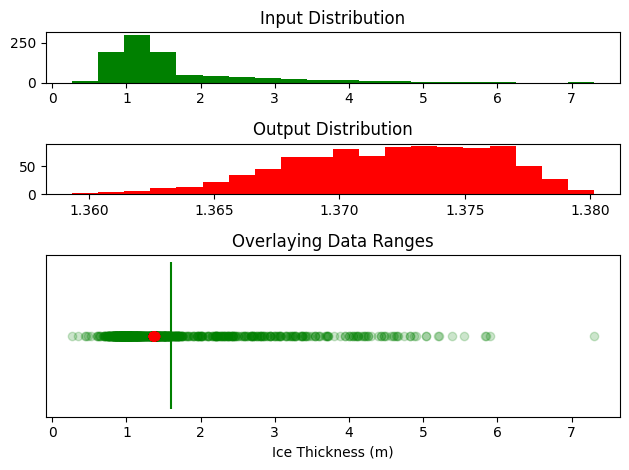
\includegraphics[width=.48\linewidth]{../research-resources/CNN/unconverged-distribution.png}}
	\caption[Model Performance]{(a) Model Convergence (b) Model Predictions}
	\label{fig:model-results}
\end{figure}

After 100 epochs, the model fails to converge (Figure 3.3). The L1 Loss function plateaus at $\approx0.66$, and the model predicts a concentrated set of values slightly lower than the test set's mean. This value can be explained by the L1 Loss function's insensitivity towards outliers, as the mean (vertical bar) would be shifted right because of the skew in the input distribution.

The model reports an R2 value of -.056 and an RMSE of 0.9996, both of which suggest the model does not fit the data at all. The normalized RMSE is 0.14, which seemingly better, is only the result of the relatively narrow range of ice thicknesses being predicted in the testing set. Minor changes to the activation function and hyper-parameters yielded no significant difference to the model's evaluation metrics, nor did they assist in loss convergence. The inadequacies demonstrated by these tests suggest a more sophisticated architecture would be needed to better associate these low-resolution 1 channel images with their interpolated thickness measurements.

% \section {U-Net}
    \chapter{Results}
\label{sec:Results}

Here you present the results of your study (if you carried out one), and any data analysis you may have performed to answer your question.
You should consider splitting the results per research question, as these are presented in the introduction

    \chapter{Discussion}
\label{sec:Discussion}
While the approach to applying IS-2's LiDAR measurements to ICEYE's SAR imaging was intuitive, there are several limitations of the experiment that should be acknowledged. These can be split into technical and conceptual limitations, where the former is responsible for immediate flaws in experimentation, and the latter can be viewed as persistent by nature of how they are related to the task. The practical implications of a working model are discussed after the limitations, and the section is concluded by future works for this project.

\section{Technical Limitations}
Limitations of the experimentation range from the data collection to the architecture and testing configuration. Firstly, the model's failure to converge was likely the result of inadequate architecture, but the restricted amount of data itself was plausibly a second limiting factor. As discussed at the end of the Data Collection section, of the 4 sponsored images delivered from ICEYE, only (Figure \ref{fig:gathered-sar-b}) appeared to be correlated closely enough with IS-2's track to be considered ground truth. Despite efforts to validate the location and concentration of sea ice in the acquisition area by using Copernicus Access Hub, the selected area was too sparse for IS-2 to deliver information from all 6 beams. The low resolution of SN-2 data via Copernicus Access Hub combined with the latency between the data order and delivery means that there is a degree of randomness with any data acquisition even when sponsored. IS-2's data delivery flagged 70$\%$ of its gathered data for the possible interference of weather, either through blowing snow or clouds. Considering IS-2's weather flag then, the original expectation of $\approx$ 11,300 tiles from the 2 SPOT and 2 SLEA images actually only produced 1,391 tiles, for a yield of 12.30$\%$.

Furthermore with the data, the coincidence of (Figure \ref{fig:gathered-sar-b}) is based on the assumption that the ice did not drift more than 17 meters within the acquisition window. Essentially, if the ice drifted even 3 $\frac{m}{min}$ it's possible for the data to be a close proxy for the ground truth, but technically incorrect altogether. Buoy data for the time frame showed that 2 buoys, 185km and 300km away were traveling at a mean speed of 12 $\frac{m}{min}$ and 16.67 $\frac{m}{min}$ respectively during the hour of acquisition. Combined with the assumed geolocation accuracy of 5m \cite{ICESat-2-Horizontal-Accuracy} and that some studies find the mean effective footprint of IS-2 to be 10.9 $\pm$ 1.2m\cite{icesatfootprintdiameter}, the assumption of coincidence becomes weaker.

Statistically, many measurements used during the study were accompanied by uncertanties, standard deviations, and confidence levels. These values were ignored during the experimentation, but should be considered in more thorough analysis in the future. 

\section{Conceptual Limitations}
The introduction discussed the assumption of hydrostatic equilibrium and associated Equation \ref{eq:isostatic-equilibrium} as an established method to deduce ice thickness from remote measurements. Like previously mentioned, there is contention between which values to use for each density. Simply by assuming the maximum and minimum of acceptable densities for sea ice and snow, the same data from the experimentation can be seen ranging over a whole meter in some places like index 1050 of the GT2R beam (Figure \ref{fig:density-bounds}). It's important to realize that this exact acquisition saw freeboard $<$ 1m, but with acquisitions of ice with more freeboard, these error bounds would increase in magnitude.

\begin{figure}[h]
	\centering
	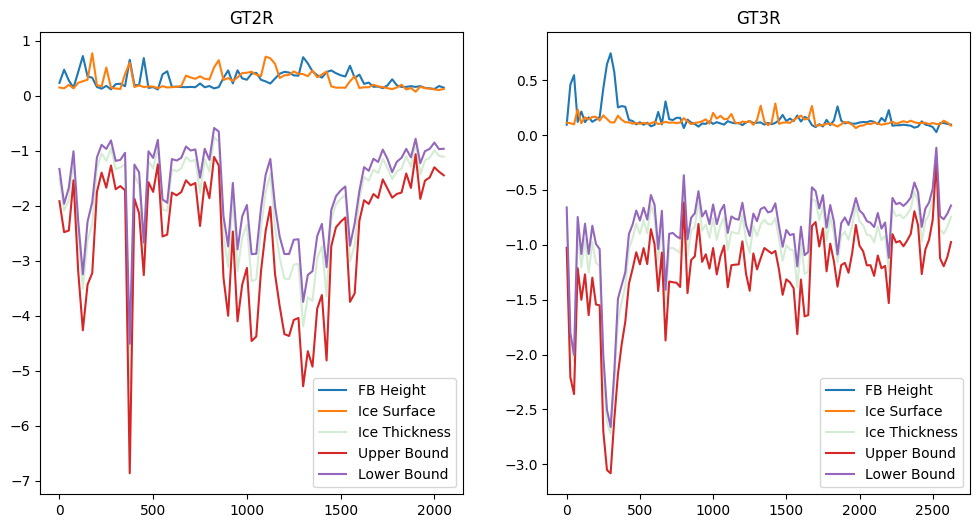
\includegraphics[width=.8\textwidth]{../research-resources/ice-sat-2/density-bounds.png}
	\caption[Effect of Density Estimations on Ice Thickness Interpolation]{Bounded Ice Thickness}
	\label{fig:density-bounds}
\end{figure}

Coupled with the issue of ice density in the hydrostatic model, is the general assumption of ice homogeneity. Equation \ref{eq:isostatic-equilibrium} demonstrates the densities involved in interpolating for sea thickness, but it's important to realize these forces are assumed to be at play on independent buoyant ice segments. In practicality, ice floes as a whole are in hydrostatic equilibrium and the point-to-point assumption used in Equation \ref{eq:isostatic-equilibrium} does not necessarily hold \cite{Forsström_Gerland_Pedersen_2011}. The differences can be results of ice deformation or composition, ridges, or even  internal shear forces \cite{Hutchings_Heil_Lecomte_Stevens_Steer_Lieser_2015,sea-ice-properties}. 

A final conceptual limitation with the corroboration of LiDAR with SAR imaging, is that the specific satellite capturing the image has a meaningful effect on the model being used. ICEYE's SAR imaging was pursued because of it's high 1m resolution. However, these images were captured using X-Band frequencies which are different from SN-2's frequencies \cite{iceye-products,Sentinel-2-Availability}. One of SAR's advantages is its ability to permeate through snow, allowing for it to capture the ice-surface below it. It's exact penetration depth though, is highly variable across the range of LiDAR and RADAR wavelengths \cite{remotesensingkinematics}. In this sense, the tiles derived from ICEYE will have to be compared to other X-Band SAR imaging satellites to ensure both images capture the same context.


\section{Practical Implications}
The development of a model like this has practical implications in both science and navigation. By tracking the thickness of ice floes across the arctic and measuring how a single floe grows or melts over time, researchers can better model the dynamics of sea ice using quantifiable changes. In the field of navigation, singular SAR images can be used to determine regions of thick and thin ice and use the information to better plan routes through arctic passages. 
\begin{figure}[h]
	\centering
	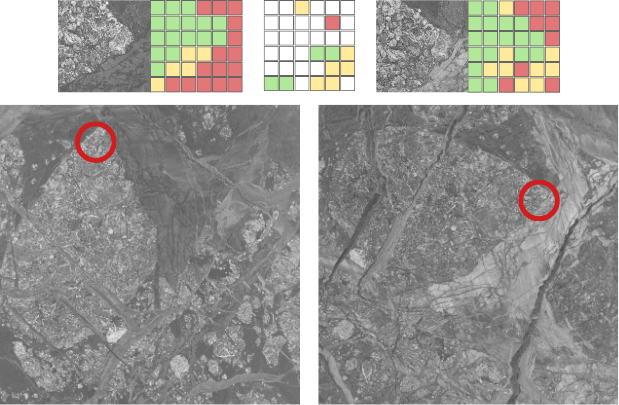
\includegraphics[width=.8\textwidth]{../images/Practical-Implications.png}
	\caption[Implications of LiDAR mapped SAR]{Change Detection between geo-located Figures 2.2(a) and 2.2(b)}
	\label{fig:change-detection}
\end{figure}


\section{Future Work}
As mentioned in the experimentation, little work has been done in regression tasked CNNs of low resolution single channel images. The difficulty in aggregating a dataset for this study suggests that this task may not be a good use case for these deep learning models, as they rely heavily on mass amounts of data. However, the U-Net architecture is one such CNN that has seen efficacy in sea ice SAR imaging, particularly in image segmentation, and could be explored in its regression capabilities on lower-resolution images \cite{SAR-U-Net}. Moving forward, pursuing ensemble learning through a more statistical approach of the low resolution data would be a valuable use of the obtained data set, and possibly more feasible than a deep learning model.

    \chapter{Conclusion}
\label{sec:Conclusion}

The result of this thesis is a rough pipeline that links elusive data to a intuitive method of better modeling sea ice. IceSat-2's semi-frequent orbit provides data that can, with planning, be corroborated with other data sources to bridge the gap between different remote sensing methods. The results of the experimentation do not suggest the model is capable of deducing sea-ice thickness from mere SAR imaging.


\section{Research Questions}
Here you will answer your research questions, as they appear in the introduction. Answer each question in a different section. Relate your answer to your results.
Discuss if your findings support and align with related work or not. Explain why do you think this happens, especially if your findings contradict existing work.
Discuss alternative interpretations of your findings.

    
%Figures, tables and references
    \cleardoublepage
    \listoffigures
    \printbibliography
  
%appendices    

    \cleardoublepage
    \pagenumbering{roman}
    \appendix
    % !TeX root = main.tex

\chapter{Insert Appendix Name}
\section{Insert subtitle}


\end{document}
